\documentclass[12pt]{article}
\usepackage[utf8]{inputenc}

\usepackage{geometry}
\geometry{a4paper, scale=0.8}

% For prettier tables
% replace \hline with \toprule, \midrule and \bottomrule
\usepackage{booktabs}

% For list spacing
\usepackage{enumitem}
\setlist{noitemsep} % or \setlist{nosep} to leave space around whole list
% \setlist{nolistsep}

% For multi-column
\usepackage{multicol}
\setlength{\columnsep}{1cm}

% For graphic/figure
\usepackage{graphicx}

\title{\textbf{SemEval-2018 Task 7 Subtask 1: Semantic Relation Classification in Scientific Papers}}
\author{\textbf{Hui-Qiang Jiang} \quad \textbf{Da-Wei Lee} \\
Peking University \\
{\tt \{1801210840,1701210963\}@pku.edu.cn}}
\date{April 9, 2019}

\begin{document}
\maketitle
\begin{abstract}
  First, we test the performance with some naive ideas to transform the problem into a trainable form. Then sifting out the unfeasible one and bad performance one. Doing some research on previous competitors' paper. Then we decide to follow the LightRel model. We looking for the most important factors that affect the performance the most. Finally, focusing on them and aim to gain more improvement on the Macro F1 score.

We achieve a 56.3\% F1 score on Task 1.1. And it beats the best performance of the LightRel 46.4\%.
\end{abstract}

\begin{multicols}{2}

\section{Introduction}


\section{Related Work}
\label{sec:related_work}

We spent much time working on how to transform the problem into a trainable form. We found that it is also very hard for a human (ourselves) to classify this task.
(And we have drawn on the experience of the other paper. )

\subsection{Naive Idea on Relation}
\label{sec:naive_idea_on_relation}

We first doing some research on semantic relation typology. There are six major relation types of this competition, USAGE, RESULT, MODEL, PART\_WHOLE, TOPIC, and COMPARISON. And each of them may have a REVERSE relation (except COMPARISON).

The idea is putting connection words between two entities. And calculate the probability of whether it matches which relation type the most.

There are the combinations we've made:

\begin{itemize}
    \item USAGE
    \begin{itemize}
        \item used by
        \item used for
        \item applied to
        \item performed on
    \end{itemize}
    \item RESULT
    \begin{itemize}
        \item affects
        \item problem
        \item yields
    \end{itemize}
    \item MODEL
    \begin{itemize}
        \item of and observed
        \item associated to
    \end{itemize}
    \item PART\_WHOLE
    \begin{itemize}
        \item composed of
        \item extracted from
        \item found in
    \end{itemize}
    \item TOPIC
    \begin{itemize}
        \item presents
        \item of
    \end{itemize}
    \item COMPARISON
    \begin{itemize}
        \item compared to
    \end{itemize}
\end{itemize}

\subsection{Improved Relation}
\label{sec:improved_relation}

We try to use the words between two entities as the basis of predicting relation. And we found that LightRel has done a similar thing.

LightRel let all the sentences with the same length (i.e. same dimension feature). But the sentence in the training and test set won't always be the same. Thus they have padded some dummy words into the sentence to fill the empty space.

We think this approach is much more reasonable than the previous one. Because the relation of any two words can easily tell by the connecting words or sentence.

\subsection{Feature Engineering}
\label{sec:feature_engineering}

We have also observed some of the training samples. And conclude some possible pattern such that if the first word is end with "'s", then it possibly has maybe a sort of belonging relation between them.

In LightRel, they have done many features, they called "word-shape feature", as well. But by our experiment, we found that. Using these features will only lower the performance. So we only use enable this as comparison purpose.

\begin{itemize}
    \item any character is capitalized
    \item a comma is present
    \item the first character is capitalized and the word is the first in the relation
    \item the first character is lower-case
    \item there is an underscore present (representing a multi-word entity)
    \item if quotes are present in the token
\end{itemize}

\subsection{Embedding}
\label{sec:embedding}

We found that the most significant improvement of the performance is related to embedding. There are two subjects: What corpus we choose to calculate the embedding. And what tools to form the embedding. We have made several tests.

\subsubsection{Corpus}
\label{sec:corpus}

We selecting the candidate corpus on the Citation Network Dataset~\footnote{https://aminer.org/citation ~\cite{Tang:08KDD}}. This dataset provides the scientific paper of recent years. LightRel chooses DBLP  v5 combined with ACM v9. And extract out only the "Abstract" part of the paper using the regular expression.

We have done some combination of selection like testing by using DBLP v5 only or using DBLP v10 combined with ACM v9 etc.

\subsubsection{Embedding Model}
\label{sec:embedding_model}

There are several tools that we have tried. Such as word2vec~\footnote{\cite{NIPS2013_5021}} by Google (also used in LightRel), fastText by Facebook and BERT by Google.

We build the embedding with 300 dimension vector and skip the words with appearance less than 5 times. We use the mean of all other embeddings to deal with the out-of-vocabulary problem (i.e. the [UNK] token).

There are some tests among these three model. The usage of the word2vec and the fastText is very similar. The BERT, because there are too many parameters, need to fine-tune to fit the problem, but we haven't found a good solution, thus the performance is not as good as the previous tools. Finally, we found that fastText perform better than others.

\section{Model and Framework}
\label{sec:model_and_framework}

The first attempt is continuing using the model used by LightRel, the logistic regression model offered by LibLinear. But to form the required format that fit LibLinear is quite handy because it needs to be file format with a kind of sparse matrix representation. That become complicated when we need to do k-fold cross-validation on the training set.

Then we tried to use Scikit Learn library. Because the API of Scikit Learn are similar so we can switch from multiple models and test the performance easily. We have tried LinearSVC, LogisticRegression and Decision TreeClassifier. And we found the LogisticRegression has still had the best performance.

In the test of LightGBM, the performance is not quite ideal. In the first case, we think that because the dimension of features is too large, using a tree-based algorithm may not be a good idea.

Finally, we have tried the simple version TextCNN model, the performance is not too bad but still lower than the statistics machine learning model. So we have deprecated it later on.

\begin{figure*}[ht]
    \begin{center}
    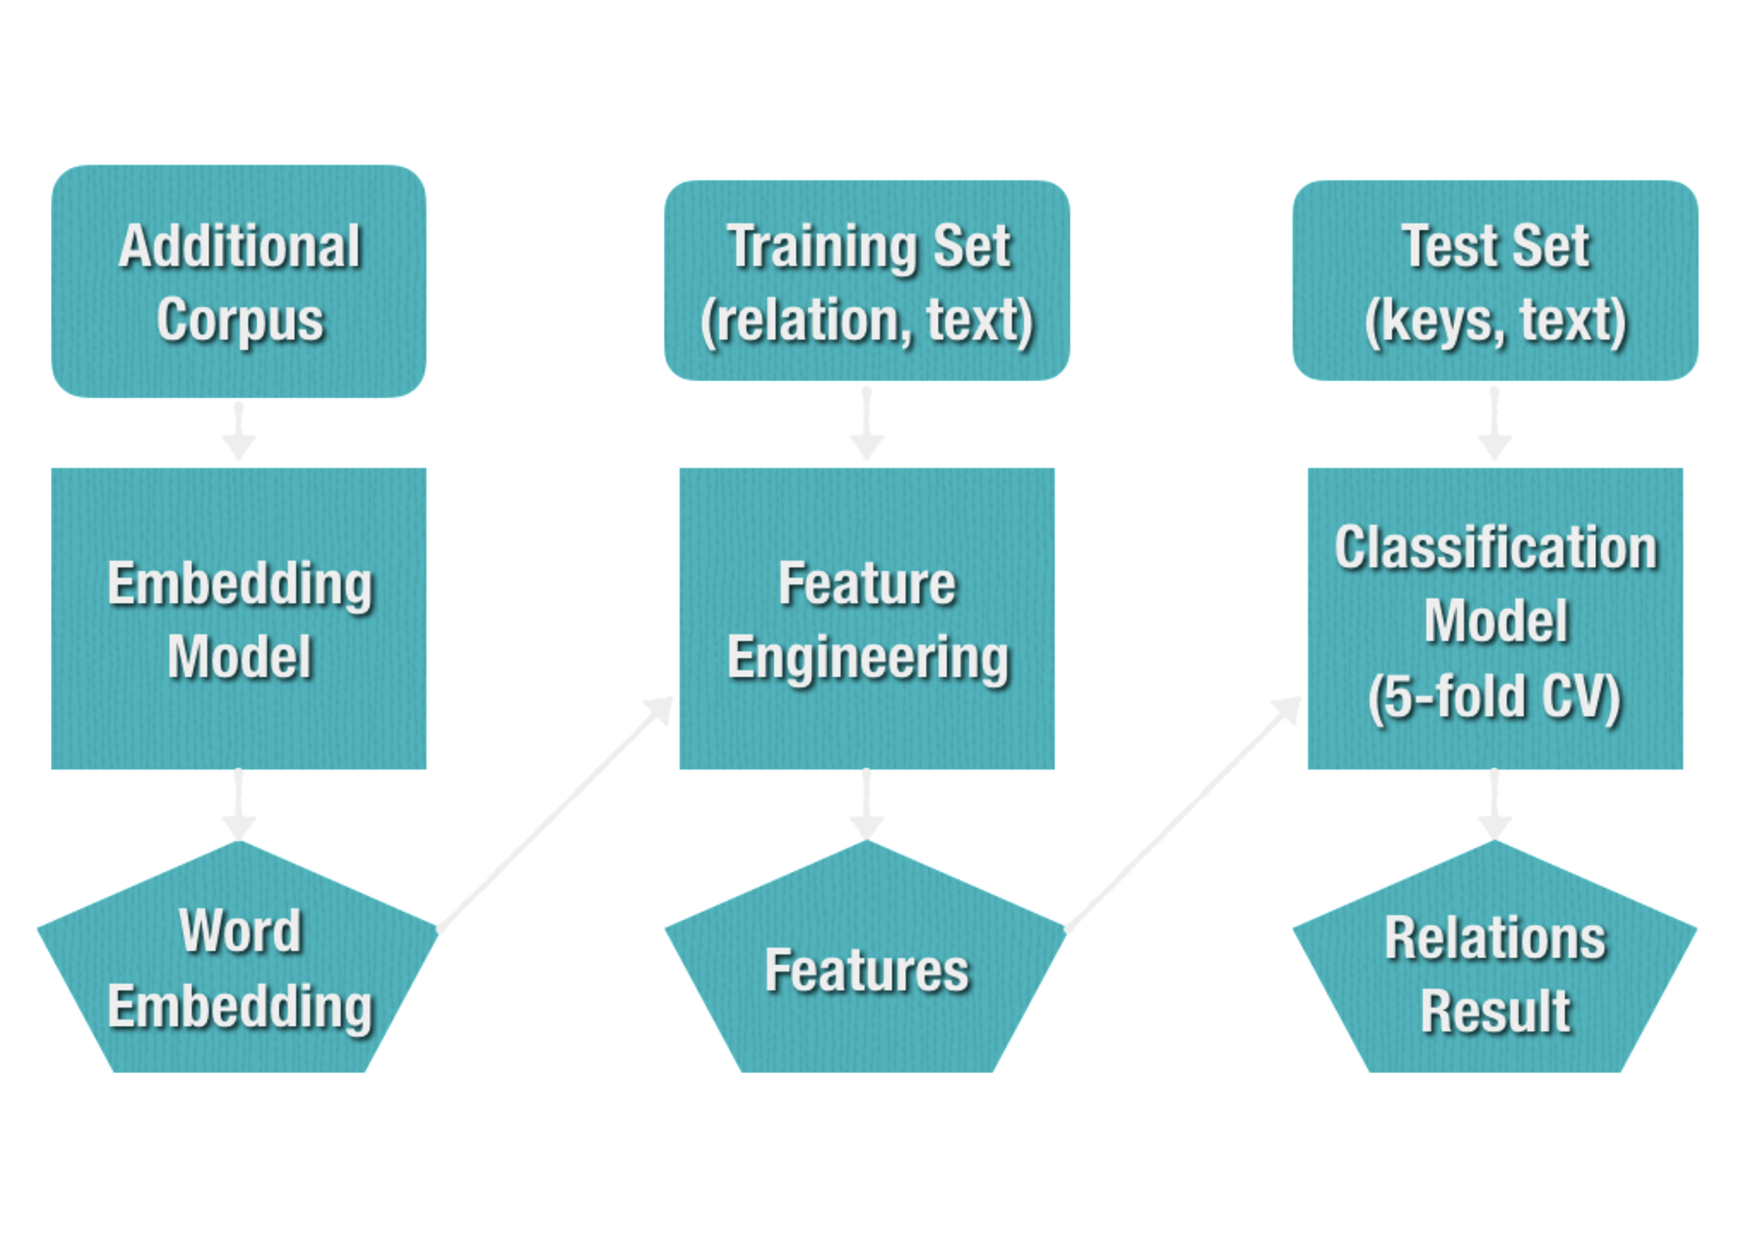
\includegraphics[width=0.85\textwidth]{figures/overall_model.pdf}
    \end{center}
    \caption{The overview of model structure}
    \label{fig:overall_model}
\end{figure*}


\end{multicols}

\section{Experiment}
\label{sec:experiment}

In the previous section, we mentioned many experiments on the different corpus, embedding tools and model. We will list the performance of each attempt and highlight the best performance on both tasks.

Because the TOPIC class in subtask 1.1 is unbalanced. So we can see the phenomenon that subtask 1.2 will overall be higher than subtask 1.1.

\subsection{Different Corpus and Embedding Model}
\label{sec:different_corpus_and_embedding_model}

Word embedding almost the important thing in NLP task. So we take some word embedding method and train dataSet to tune the effect of word embedding.

First of all, the train dataSet of competition is so small that the effect of training word embedding is bad. So we import some outer dataSet to optimization the effect of word embedding. The domain of our task is about scientific papers. So, we load dataset on Citation Network Dataset. We test dblp v5, dblp v10, and acm v9, we find dblp v10 have best f1 score both in trainSet and testSet.

We also do some work on different word embedding methods, like word2vec, Bert, fastText. FatsText do the best job in our experiment. Bert doesn't have a good effect on our task. We think it may be caused by the embedding size of the pre-train model.

\begin{table}[htbp!] % here top bottom page (! = remove further restrictions)
    \begin{tabular}{llcccc}
    \toprule
        \multicolumn{2}{c}{Task}                                                 & \multicolumn{2}{c}{Subtask 1.1} & \multicolumn{2}{c}{Subtask 1.2} \\
    \midrule
        Corpus & Embedding Model                                                               & Macro-F1        & Micro-F1       & Macro-F1        & Micro-F1       \\
    \midrule
        Pre-trained DBLP v5 & word2vec    & 88.99            & 78.99           & 64.99            & 38.99           \\
        ACM v9 + DBLP v10   & word2vec & 87.99            & 78.99           & 64.99            & 38.99           \\
        DBLP v5   & word2vec & 87.99            & 78.99           & 64.99            & 38.99           \\
        DBLP v10   & word2vec & 87.99            & 78.99           & 64.99            & 38.99           \\
        ACM v9 + DBLP v10   & fastText & 87.99            & 78.99           & 64.99            & 38.99           \\
        DBLP v10   & fastText & 87.99            & 78.99           & 64.99            & 38.99           \\
        ACM v9 + DBLP v10   & BERT & 87.99            & 78.99           & 64.99            & 38.99           \\
    \bottomrule
    \end{tabular}
\caption{Comparison between different corpus using LibLinear logistic regression model (in \%)}
\label{tab:corpus}
\end{table}


\subsection{Different Feature}
\label{sec:different_feature}

We also do some work on feature engineering. We test the effect of different '[PAD]' position. Clustering is also one way to improve our model. We add both one-hot and word embedding of middle words between two entities to feature lists. And we also do some artificial features like have including '\_' in middle words between two entities. We do some experiment which one by one add features to model.

\begin{table}[htbp!] % here top bottom page (! = remove further restrictions)
    \centering
    \begin{tabular}{lccccc}
    \toprule
        \multicolumn{2}{c}{Task}                            & \multicolumn{2}{c}{Subtask 1.1 Test}  & \multicolumn{2}{c}{Subtask 1.1 Training} \\
    \midrule
        Model & Feature                                     & Macro-F1         & Micro-F1           & Macro-F1         & Micro-F1       \\
    \midrule
        LibLinear\\ Logistic Regression    & embedding only & \bf52.01         & -                  & 49.97            & -              \\
        LibLinear\\ Logistic Regression    & + one-hot      & 51.43            & -                  & 49.25            & -              \\
        LibLinear\\ Logistic Regression    & + shape        & 50.61            & -                  & 49.67            & -              \\
        LibLinear\\ Logistic Regression    & + cluster      & 51.55            & -                  & 49.31            & -              \\
        LibLinear\\ Logistic Regression    & + e1, e2       & 49.93            & -                  & 49.97            & -              \\
        Scikit Learn\\ Logistic Regression & embedding only & 50.37            & -                  & 52.12            & -              \\
        Scikit Learn\\ Logistic Regression & + one-hot      & 51.10            & -                  & 52.37            & -              \\
        Scikit Learn\\ Logistic Regression & + shape        & 51.29            & -                  & 51.81            & -              \\
        Scikit Learn\\ Logistic Regression & + cluster      & 51.90            & -                  & 51.97            & -              \\
        Scikit Learn\\ Logistic Regression & + e1, e2       & 50.92            & -                  & \bf52.99         & -              \\
    \bottomrule
    \end{tabular}
\caption{Comparison between differen feature based on LibLinear and Scikit Learn logistic regression model (in \%)}
\label{tab:feature}
\end{table}


\subsection{Different Model}
\label{sec:different_model}

Except for linear regression model, we also do some experiment on SVM, LinerSVC,DecisionTreeClassifier , TextCNN.

\begin{enumerate}
    \item Linear Regression use L2-regularized logistic regression type, cost=0.05, epsilon=0.1
    \item SVM use L2-penalty, squared hinge as loss function, C=1.0, OVR on multi-classification
    \item Decision Tree use gini impurity as criterion, max depth=$\infty$, min sample split=2
    \item TextCNN use 128 filter, filter size=[6,7,8], embedding size=300, learning rate = 0.0003, batch size = 64, decay step=1000, train around 300epochs, we get a local optimum train f1 score.
\end{enumerate}

\begin{table}[htbp!] % here top bottom page (! = remove further restrictions)
    \centering
    \begin{tabular}{lcccc}
    \toprule
        \multicolumn{1}{c}{Task}           & \multicolumn{2}{c}{Subtask 1.1}    & \multicolumn{2}{c}{Subtask 1.2}    \\
    \midrule
        Model Name                         & Macro-F1         & Micro-F1        & Macro-F1         & Micro-F1        \\
    \midrule
        LibLinear\\ Logistic Regression    & 52.01            & -               & 69.15            & \bf81.41        \\
        Scikit Learn\\ Logistic Regression & \bf52.77         & -               & 75.06            & 76.04           \\
        Scikit Learn\\ Linear SVM          & 51.45            & -               & 70.29            & 75.56           \\
        Scikit Learn\\ Decision Tree       & 36.65            & -               & -                & -               \\
        TextCNN                            & 51.20            & 65.50           & \bf77.35         & 80.53           \\
    \bottomrule
    \end{tabular}
\caption{Comparison between differen machine learning model using fastText embedding model on DBLP v10 corpus (in \%)}
\label{tab:model}
\end{table}


\begin{figure*}[ht]
    \begin{center}
    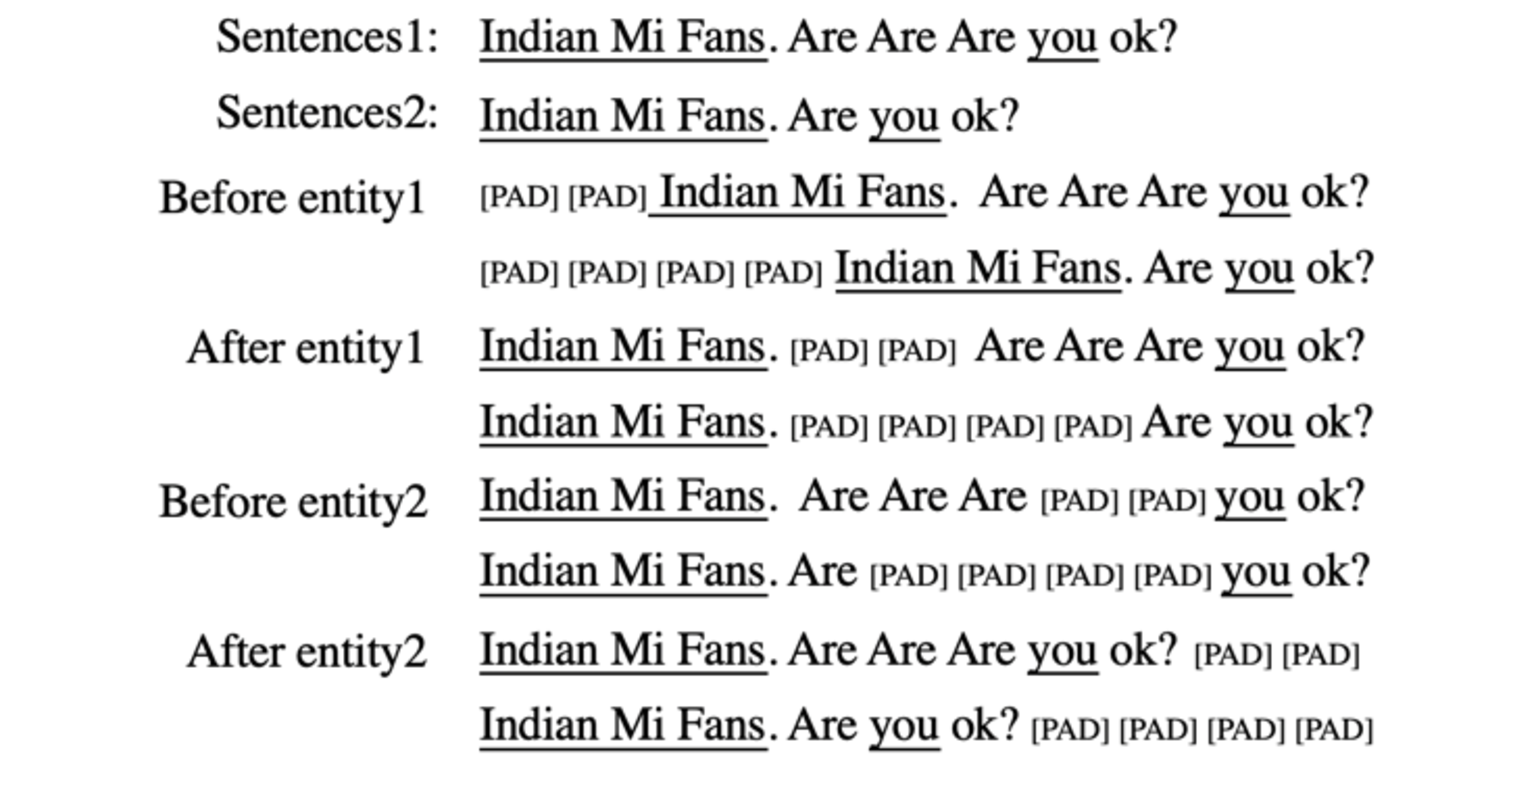
\includegraphics[width=0.85\textwidth]{figures/pad_example.pdf}
    \end{center}
    \caption{Pad example (MAX sentences size = 12)}
    \label{fig:pad_example}
\end{figure*}


\subsection{Imbalance Data}
\label{sec:impalance_data}

The train dataset is an obvious imbalance set in subtask 1.1 Topic class. So we over-sampling the train set. We, in turn, add subtask 1.2 Train Topic, subtask 1.2 Test topic, subtask 1.2 Train, subtask 1.2 Test, subtask 1.2 to subtask1.1. And test the effect of over-sampling.

\begin{table}[htbp!] % here top bottom page (! = remove further restrictions)
    \begin{tabular}{lccccc}
    \toprule
        \multicolumn{1}{c}{Training Data}            & \multicolumn{2}{c}{Subtask 1.1 Test}  & \multicolumn{2}{c}{Subtask 1.1 Training} \\
    \midrule
        Training Data                                & Macro-F1         & Micro-F1           & Macro-F1         & Micro-F1       \\
    \midrule
        only subtask 1.1 training data               & 50.92            & 65.17              & 52.99            & -              \\
        + subtask 1.2 TOPIC data                     & 50.20            & 64.41              & 52.62            & -              \\
        + subtask 1.2 and test set TOPIC data        & 50.50            & 68.12              & 46.22            & -              \\
        + all the subtask 1.2 data                   & \bf53.73         & \bf71.07           & \bf67.20         & -              \\
        + all the test data                          & 52.82            & 68.26              & 66.73            & -              \\
        + everything                                 & 52.82            & 70.22              & 66.42            & -              \\
    \bottomrule
    \end{tabular}
\caption{Comparison between using different training data on Scikit Learn logistic regression model in order to solve the data imbalance problem on subtask 1.1 (in \%)}
\label{tab:data_imbalance}
\end{table}


The evaluation shows that class imbalance impacts the effect of subTask 1.1. But more data don't mean a better effect. When we add all data of subTask 1.2 including task and train data, we found the effect is worse than data fusing only subTask1.2 train data. And the over-sampling Topic class is not significant.

\subsection{Pad Position}
\label{sec:pad_position}

The lens between two entities is different in dataSet. So we should align word list before all word. We can put '[PAD]' before the entity1, after entity1, before entity2, after entity2. The result of 4 methods should be different. So we take some experimentation to explore this problem. We use TextCNN with Task1.1+Task1.2 Train dataSet, use 128 filters, filter size=[6,7,8], embedding size=300, learning rate = 0.0003, batch size = 64, decay step=1000.

\begin{table}[htbp!] % here top bottom page (! = remove further restrictions)
    \begin{tabular}{lccccc}
    \toprule
        \multicolumn{1}{c}{Training Data}          & \multicolumn{2}{c}{Subtask 1.1 Test}  & \multicolumn{2}{c}{Subtask 1.2 Test} \\
    \midrule
        Pad Position                               & Macro-F1         & Micro-F1           & Macro-F1         & Micro-F1       \\
    \midrule
        pad before entity1                         & 59.74            & 66.95              & 71.22            & 77.29         \\
        pad after entity1                          & 56.79            & 66.67              & 72.76            & 80.79         \\
        pad before entity2                         & \bf67.74         & \bf72.03           & \bf73.03         & \bf81.01      \\
        pad after entity2                          & 57.70            & 65.63              & 72.48            & 80.23         \\
    \bottomrule
    \end{tabular}
\caption{Comparison between padding different position on TextCNN model and use subtask 1.1 + subtask 1.2 training data to show the effect (in \%)}
\label{tab:data_pad}
\end{table}


The evaluation shows that padding position is a vital parameter in our model. In all subTask, we found that adding pad before entity1 is a good way to improve the performance of our model.

\section{Conclusion and Future Work}

\bibliographystyle{acl_natbib}
\bibliography{mybib}

\end{document}
